\documentclass{article}%
\usepackage[T1]{fontenc}%
\usepackage[utf8]{inputenc}%
\usepackage{lmodern}%
\usepackage{textcomp}%
\usepackage{lastpage}%
\usepackage{authblk}%
\usepackage{graphicx}%
%
\title{Expression of bovine (Bos indicus) interleukin{-}18 in Escherichia coli and its biological activity}%
\author{Brian Savage}%
\affil{Oncology Research, Pfizer Worldwide Research and Development, San Diego, California, United States of America}%
\date{01{-}01{-}2014}%
%
\begin{document}%
\normalsize%
\maketitle%
\section{Abstract}%
\label{sec:Abstract}%
Please enable Javascript to watch this video\newline%
SAN DIEGO {-}{-} Scientists believe the study highlights the potential benefits of high{-}expressing, billion{-}fold{-}cell doubling biological complexes like Uev1A{-}Ubc13, which has been shown to be helpful in cell development and cancer treatment.\newline%
"This study shows that adding Uev1A{-}Ubc13 to a baker's block genetically enhanced like Uev1A{-}Ubc13 causes estrogen{-} and progesterone{-}like changes which strongly promote tumor formation and metastasis in breast and prostate cancer cells," said Sue Lee, professor of ophthalmology at UC San Diego.\newline%
Lee and her colleagues exposed cells from mice to high levels of Uev1A{-}Ubc13, which elevated gene expression through ion channels.\newline%
They found that the new, "drug analog" cell continues to shift from the same tumor{-}signaling pathway and is more like a tumor{-}ridden lab dish.\newline%
Further tests indicate that Uev1A{-}Ubc13 is one of the first biological complexes to be validated as a replacement for transmembrane DNA{-}binding structures that are intended to reduce cancer proliferation.\newline%
The findings have been published in the Proceedings of the National Academy of Sciences.\newline%
Researchers also believe the findings indicate a breakthrough in treating breast cancer with "herbs," which act as target molecules to kill cancer cells by increasing their cellular uptake and cell proliferation.\newline%
Lee and her colleagues hope to utilize this new study to translate Uev1A{-}Ubc13 onto human epithelial cells where it could be used to combat certain types of breast cancer.

%
\subsection{Image Analysis}%
\label{subsec:ImageAnalysis}%


\begin{figure}[h!]%
\centering%
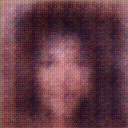
\includegraphics[width=150px]{500_fake_images/samples_5_411.png}%
\caption{A Black Cat Sitting On Top Of A Window Sill}%
\end{figure}

%
\end{document}